\documentclass[tikz,border=12pt]{standalone}
\usepackage[utf8]{inputenc}
\usepackage[T1]{fontenc}
\usepackage{helvet}
\renewcommand{\familydefault}{\sfdefault}
\usetikzlibrary{arrows.meta,calc,fit,backgrounds}

\tikzset{
	inp/.style={draw=black, rounded corners=4pt, fill=gray!65, text=white,
		minimum width=1.7cm, minimum height=0.62cm, line width=0.6pt},
	hid/.style={draw=black, rounded corners=4pt, fill=gray!50,
		minimum width=1.7cm, minimum height=0.62cm, line width=0.6pt},
	outw/.style={draw=black, rounded corners=4pt, fill=gray!15, text=black,
		minimum width=1.7cm, minimum height=0.62cm, line width=0.6pt},
	blk/.style={draw=black, rounded corners=10pt, line width=0.9pt,
		inner xsep=12pt, inner ysep=12pt},
	rowlab/.style={anchor=east, font=\small},
	title/.style={font=\Large},
	note/.style={font=\bfseries\small, align=center},
	arr/.style={-{Stealth[length=2.4mm]}, line width=0.8pt},
}

\newcommand{\dx}{2.6}

\begin{document}
	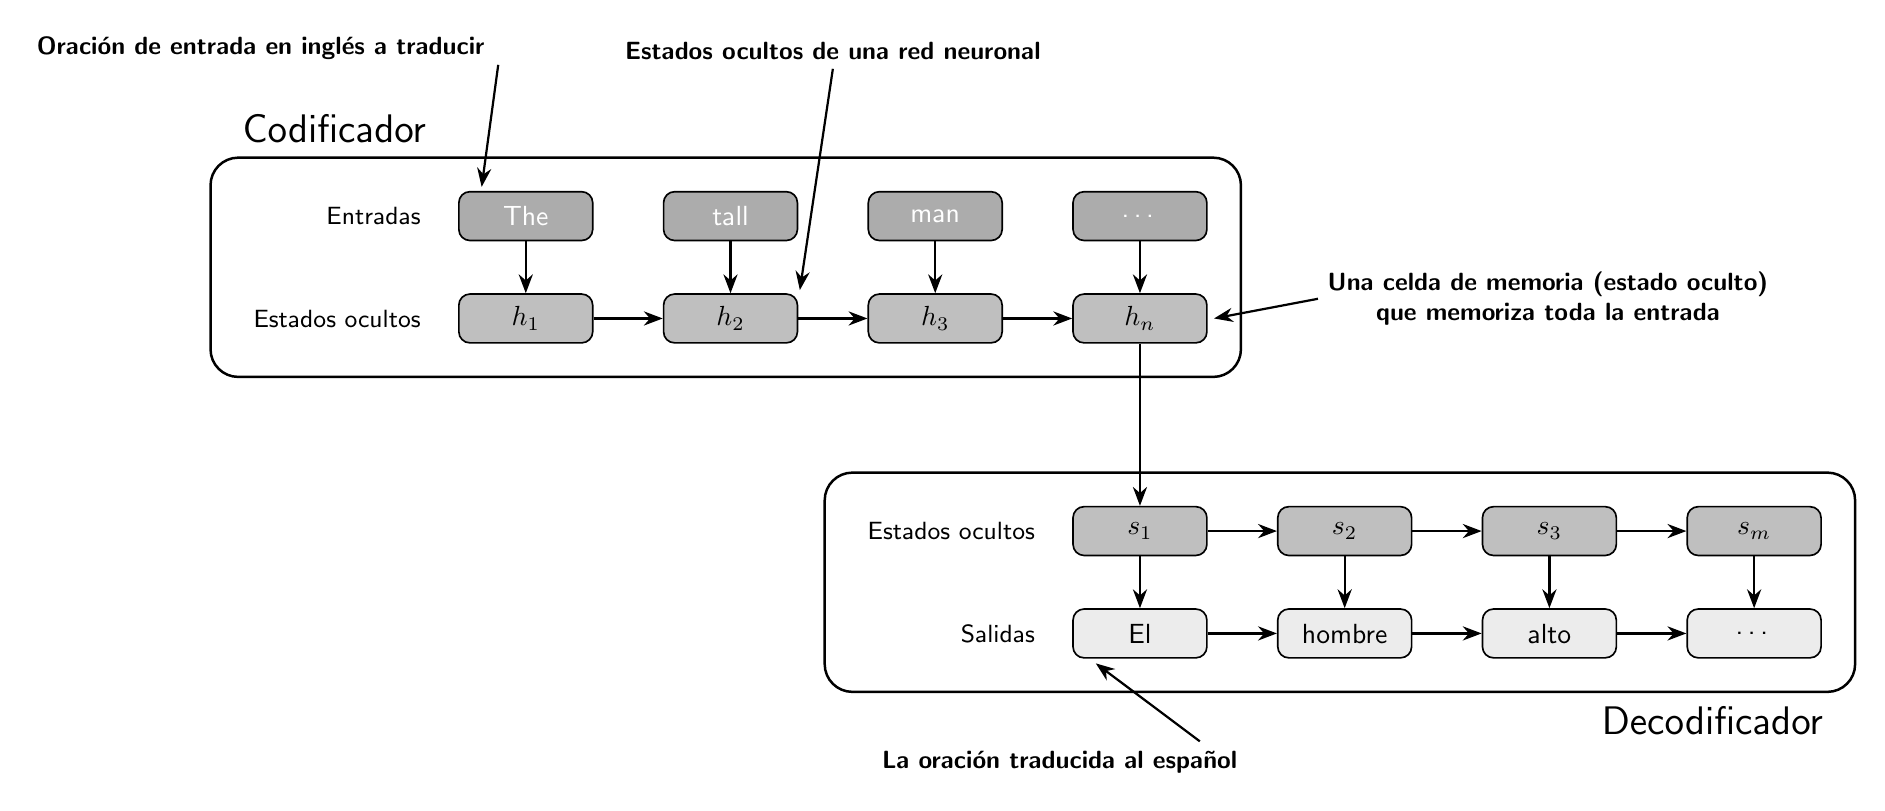
\begin{tikzpicture}
		
		%% ============================ Codificador (arriba) ============================
		\foreach \w [count=\i] in {The,tall,man,\dots}
		\node[inp] (x\i) at ({(\i-1)*\dx},0) {\w};
		\foreach \lab [count=\i] in {h_1,h_2,h_3,h_n}
		\node[hid] (h\i) at ({(\i-1)*\dx},-1.3) {$\lab$};
		
		\foreach \i in {1,...,4}
		\draw[arr] (x\i.south) -- (h\i.north);
		\foreach \i/\j in {1/2,2/3,3/4}
		\draw[arr] (h\i.east) -- (h\j.west);
		
		\node[rowlab] (lx) at ($(x1.west)+(-0.35,0)$) {Entradas};
		\node[rowlab] (lh) at ($(h1.west)+(-0.35,0)$) {Estados ocultos};
		
		\begin{scope}[on background layer]
			\node[blk, fit=(lx)(lh)(x4)(h4)] (enc) {};
		\end{scope}
		\node[title, anchor=south west] at ($(enc.north west)+(0.3,0.05)$) {Codificador};
		
		%% =========================== Decodificador (abajo) ===========================
		\def\yd{-4.0}
		\foreach \lab [count=\i] in {s_1,s_2,s_3,s_m}
		\node[hid] (s\i) at ({(\i+2)*\dx},\yd) {$\lab$};
		\foreach \w [count=\i] in {El,hombre,alto,\dots}
		\node[outw] (y\i) at ({(\i+2)*\dx},\yd-1.3) {\w};
		
		\foreach \i in {1,...,4}
		\draw[arr] (s\i.south) -- (y\i.north);
		\foreach \i/\j in {1/2,2/3,3/4}
		\draw[arr] (s\i.east) -- (s\j.west);
		\foreach \i/\j in {1/2,2/3,3/4}
		\draw[arr] (y\i.east) -- (y\j.west);
		
		\node[rowlab] (ls) at ($(s1.west)+(-0.35,0)$) {Estados ocultos};
		\node[rowlab] (ly) at ($(y1.west)+(-0.35,0)$) {Salidas};
		
		\begin{scope}[on background layer]
			\node[blk, fit=(ls)(ly)(s4)(y4)] (dec) {};
		\end{scope}
		\node[title, anchor=north east] at ($(dec.south east)+(-0.3,-0.05)$) {Decodificador};
		
		%% Único vector de contexto: el último estado oculto del codificador
		\draw[arr] (h4.south) -- (s1.north);
		
		%% =============================== Anotaciones ================================
		\node[note, anchor=south east] (n1) at ($(x1.north)+(-0.4,1.55)$)
		{Oración de entrada en inglés a traducir};
		\draw[arr] ($(n1.south east)+(0.05,0.05)$) -- ($(x1.north west)+(0.3,0.05)$);
		
		\node[note, anchor=south] (n2) at ($(x2.north)+(1.3,1.55)$)
		{Estados ocultos de una red neuronal};
		\draw[arr] ($(n2.south)+(0,0)$) -- ($(h2.north east)+(0.02,0.04)$);
		
		\node[note, anchor=west] (n3) at ($(h4.east)+(1.4,0.25)$)
		{Una celda de memoria (estado oculto)\\que memoriza toda la entrada};
		\draw[arr] (n3.west) -- ($(h4.east)+(0.08,0)$);
		
		\node[note, anchor=north west] (n4) at ($(y1.south)+(-3.4,-1.05)$)
		{La oración traducida al español};
		\draw[arr] ($(n4.north east)+(-0.6,0)$) -- ($(y1.south west)+(0.3,-0.06)$);
		
	\end{tikzpicture}
\end{document}